\documentclass[border=0pt]{standalone}
\usepackage{amsmath}
\usepackage[usenames,dvipsnames]{xcolor}
\usepackage{graphicx}

%%font
\usepackage{euler}
\usepackage[OT1]{eulervm}
\renewcommand{\rmdefault}{pplx}

\usepackage{amsmath, amssymb}
\newcommand{\mptn}{\mathcal{S}}
\newcommand{\mptncl}{\mathcal{S}^{\rm cl}}
\newcommand{\msym}{\operatorname{Sym}_n(\mathbb{R})}
\newcommand{\mskew}{\operatorname{Skew}_n(\mathbb{R})}


\usepackage{tikz}
\tikzset{roundnode/.style={circle,draw=black,fill=blue!20}, 
every label/.style={rectangle, draw=none}}
\definecolor{TortugaColor}{rgb}{0.1,0.4,0.3}
\definecolor{Totemblue}{HTML}{09182F}
\definecolor{Totemred}{HTML}{2B030B}
\definecolor{Totemyellow}{HTML}{AD901B}
\usetikzlibrary{intersections}
%\usetikzlibrary{fadings}
\usetikzlibrary{arrows}
%\usetikzlibrary{arrows.meta}
%\usetikzlibrary{decorations}
\usetikzlibrary{decorations.pathmorphing}
\usetikzlibrary{decorations.text}
%\usetikzlibrary{fit}
%\usetikzlibrary{calc}
%\usetikzlibrary{through}
%\usetikzlibrary{positioning}
%\usetikzlibrary{graphs}
%\usetikzlibrary{mindmap}
%\usetikzlibrary{backgrounds}
%\usetikzlibrary{calligraphy}
%% \usepgfmodule{nonlineartransformations}
%% \usetikzlibrary{curvilinear}

%%% Set up polar step (code from the pgd manual)
%\makeatletter
%\def\polartransformation{%
% \pgf@x will contain the radius
% \pgf@y will contain the distance
%\pgfmathsincos@{\pgf@sys@tonumber\pgf@x}%
% pgfmathresultx is now the cosine of radius and
% pgfmathresulty is the sine of radius
%\pgf@x=\pgfmathresultx\pgf@y%
%\pgf@y=\pgfmathresulty\pgf@y%
%}
%\makeatother

\pgfdeclarelayer{background}
\pgfdeclarelayer{alpha}
\pgfdeclarelayer{beta}
\pgfsetlayers{background,alpha,main,beta}

%%pic TaiJi
\tikzset{
TaiJi/.pic={
\begin{scope}[thick,yi/.style={radius=0.4cm}]
\shade [draw=black] (0,0) circle [radius =3];
\shade [top color=black, bottom color=black!50,draw=black] (0,-3) arc [radius=3, start angle=-90, end angle=90]
arc [radius=1.5, start angle=90, end angle=270]
arc [radius=1.5, start angle=90, end angle=-90];
\draw[thin,fill=black] (0,-1.5) circle [yi];
\draw[thin,fill=white] (0,1.5) circle [yi];
\end{scope}
}}

%%pic Totu
\tikzset{
totu/.pic={
\begin{scope}[scale=0.2]
\pgfmathsetmacro{\legwidth}{0.4*0.2}
\draw[fill=green!60!black!30] (0,0.8) circle [x radius=0.3,y radius=0.4];
\foreach \i in {-1,1}{
\begin{scope}[xscale=\i]
\path (0.8,0) edge[draw=green!60!black!30,line width=\legwidth cm,line cap=round,bend left] ++(0.6,0);
\path (0.6,-1) edge[draw=green!60!black!30,line width=\legwidth cm,line cap=round] ++ (0.4,-0.4);
\end{scope}
}
\draw (0,-1.4) edge[draw=green!60!black!30,line width=\legwidth cm,line cap=round] ++ (0,-0.4);
\draw[fill=green!60!black,rounded corners] (1,0) -- (0,0.5) -- (-1,0) -- (-0.8,-1.2) -- (0,-1.6) -- (0.8,-1.2) -- cycle;
\end{scope}
}}

%%pic Rescuer
\tikzset{
Rescuer/.pic={
\begin{scope}[shift={(6.35,1.2)}]
\draw[fill=black!20!red!60!yellow] (-7,-0.8) -- (-6.7,-1.2) -- (-6,-1.2) -- (-5.7,-0.8) .. controls +(-0.3,-0.1) and +(0.3,-0.1) ..  cycle;
\end{scope}
}}

%%pic SatanHeart
\tikzset{
SatanHeart/.pic={
\pgfmathsetmacro{\SatanHradius}{1}
\pgfmathsetmacro{\LSatanHradius}{1.05}
\begin{scope}[very thick]
\draw[gray!80!blue, line width=2pt] (0,0) circle[radius=\LSatanHradius cm];
\draw[gray!80!blue] (-90:\SatanHradius) -- (-306:\SatanHradius) -- (-162:\SatanHradius) -- (-378:\SatanHradius) -- (-234:\SatanHradius) -- cycle;
\end{scope}
}}

%%pic Stone Gate
\tikzset{
stonegate/.pic={
\begin{scope}[gray]
\draw[fill,draw=none,rounded corners] (-1.3,-0.3) rectangle (-0.7,2);
\draw[fill,draw=none,rounded corners] (0.7,-0.3) rectangle (1.3,2);
\draw[fill,draw=none] (0,2) ellipse[x radius=2cm, y radius=0.3cm];
\end{scope}
}}
 
%%pic Ateles Zombia
\tikzset{
zombia/.pic={
\pgfmathsetmacro{\zombiascale}{0.2}
\begin{scope}[scale=\zombiascale]
\pgfmathsetmacro{\zombiawidth}{\zombiascale *0.3 cm}
\pgfmathsetmacro{\zombiabigcorner}{\zombiascale *4 pt}
\pgfmathsetmacro{\zombiasmallcorner}{\zombiascale *0.2 cm}
\begin{scope}[gray!40, rounded corners=\zombiabigcorner, line width=\zombiawidth, line cap=round]
%\node[circle,draw,thin] at (0,0) {};
\draw [fill,thin] (-1.9,0.4) circle [radius=0.3cm];
\draw (-1.8,0.1) -- (-2.2,-0.3) -- (-2.7,-0.6);
\draw (-1.8,0.1) -- (-1.6,-0.8) -- ++ (0.1,-0.1);
\draw (-1.8,0.1) -- (-0.9,0.1) -- (0.4,0.8);
\draw[rounded corners=\zombiasmallcorner] (0.4,0.8) -- ++ (0.3,0.2) -- ++ (0.2,-0.2);
\draw (0.7,1) -- (0.9,1.3) -- (1,2.5) -- (1.3,3) -- (1.8,2.9);
\draw (0.9,0.8) -- (0.9,0.5) -- (0.95,-0.3) -- (0.8,-1.1);
\draw (0.8,0.8) -- (0.4,0.6) -- (0,-0.7) -- ++(-0.2,-0.2);
\end{scope}
\end{scope}
}
}

%%pic family
\tikzset{
family/.pic={
\begin{scope}[xshift=-1cm]
\clip (0,0) rectangle (2,1);
\draw[fill] (0.25,0.7) circle [radius=0.1cm];
\draw[line cap=round,line width=0.06cm] (0.25,0.7) -- (0.25,0.2);
\draw[line cap=round,line width=0.06cm] (0.15,0) -- (0.25,0.2) -- (0.35,0);

\draw[fill] (0.75,0.6) circle [radius=0.1cm];
\draw[line cap=round,line width=0.06cm] (0.75,0.6) -- (0.75,0.2);
\draw[line cap=round,line width=0.06cm] (0.65,0) -- (0.75,0.2) -- (0.85,0);

\draw[fill] (1.25,0.6) circle [radius=0.1cm];
\draw[line cap=round,line width=0.06cm] (1.25,0.6) -- (1.25,0.2);
\draw[line cap=round,line width=0.06cm] (1.15,0) -- (1.25,0.2) -- (1.35,0);

\draw[fill] (1.75,0.65) circle [radius=0.1cm];
\draw[line cap=round,line width=0.06cm] (1.75,0.65) -- (1.75,0.2);
\draw[line cap=round,line width=0.06cm] (1.65,0) -- (1.75,0.2) -- (1.85,0);

\draw[line cap=round, line width=0.06cm] (0,0.3) -- (0.25,0.5) -- (0.5,0.3) -- (0.75,0.4) -- (1,0.3) -- (1.25,0.4) -- (1.5,0.3) -- (1.75,0.45) -- (2,0.3);
\end{scope}
}
}

\parindent=0pt

\begin{document}
%%2021NewYear
%% 16:9
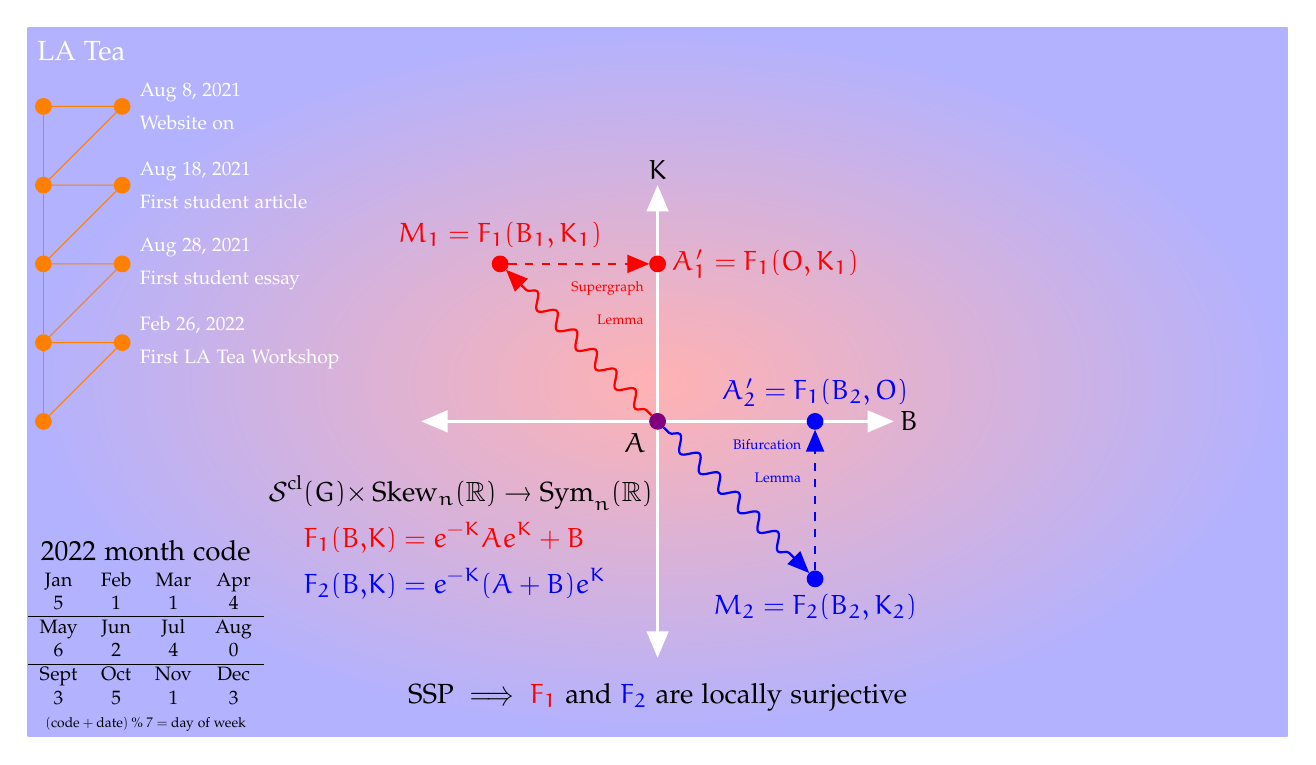
\begin{tikzpicture}
\coordinate (Jamaica) at (-8,-4);
\coordinate (Dominican) at (8,-4);
\coordinate (Cuba) at (-8,5);
\coordinate (TurksCaicos) at (8,5);
\coordinate (Tortuga) at (0,0);
\clip (Jamaica) rectangle (TurksCaicos);

%%Help Lines
\begin{pgfonlayer}{beta}
%% \draw [step=1, black!50, thin] (Jamaica) grid (TurksCaicos);
%% \draw (0,0) circle [radius=0.2cm];
\end{pgfonlayer}


%%background Layer
\begin{pgfonlayer}{background}
%% \shade [inner color=orange, outer color=red!70] (-8,-4) rectangle (8,5);
%% \shade [left color=orange, right color=red!70] (-8,-4) rectangle (8,5);
\shade [inner color=red!30, outer color=blue!30] (-8,-4) rectangle (8,5);
\end{pgfonlayer} 


%%Main Layer (main)
\begin{pgfonlayer}{main}

%%% SUPER & BIFUR
\begin{scope}
[every node/.style={circle, draw, inner sep=2pt}]
\draw[white, triangle 45 - triangle 45, very thick] (-3,0) -- (3,0);
\draw[white, triangle 45 - triangle 45, very thick] (0,-3) -- (0,3);
\node[draw=none, rectangle, right] at (3,0) {$B$};
\node[draw=none, rectangle, above] at (0,3) {$K$};

\node[label={225:$A$}, draw=red!50!blue, fill=red!50!blue] (A) at (0,0) {};

\begin{scope}[red]
\node[label={above:$M_1 = F_1(B_1,K_1)$}, fill] (M1) at (-2,2) {};
\node[label={right:$A'_1 = F_1(O,K_1)$}, fill] (A1p) at (0,2) {};
\draw[thick, decorate, decoration={snake, pre length=0.1cm, post length=0.3cm}, -triangle 45] (A) -- (M1);
\draw[thick, dashed, -triangle 45] (M1) -- (A1p);
\node[left, rectangle, draw=none, align=right] at (-0.1,1.5) {\tiny Supergraph\\ \tiny Lemma};
\end{scope}

\begin{scope}[blue]
\node[label={below:$M_2 = F_2(B_2,K_2)$}, fill] (M2) at (2,-2) {};
\node[label={above:$A'_2 = F_1(B_2,O)$}, fill] (A2p) at (2,0) {};
\draw[thick, decorate, decoration={snake, pre length=0.1cm, post length=0.3cm}, -triangle 45] (A) -- (M2);
\draw[thick, dashed, -triangle 45] (M2) -- (A2p);
\node[left, rectangle, draw=none, align=right] at (1.9,-0.5) {\tiny Bifurcation\\ \tiny Lemma};
\end{scope}

\node[rectangle, draw=none] at (-2.5,-1.5) {$
\begin{aligned}
\mptncl(G) \times &\mskew \rightarrow \msym \\
 \color{red} F_1(B, & \color{red} K) = e^{-K}Ae^K + B \\
 \color{blue} F_2(B, & \color{blue} K) = e^{-K}(A + B)e^K \\
\end{aligned}
$};

\node[rectangle, draw=none] at (0,-3.5) {SSP $\implies$ {\color{red}$F_1$} and {\color{blue}$F_2$} are locally surjective};
\end{scope}

%%% LA TEA & LA notebook
\begin{scope}
\begin{scope}[orange, shift={(-7.8,4)}, 
every node/.style={circle, draw, fill, inner sep=2pt}]
\foreach \i in {1,2,3,4,5} {
    \pgfmathsetmacro{\y}{-int(\i - 1)}
    \node (ll\i) at (0,\y) {};
}
\foreach \i in {1,2,3,4} {
    \pgfmathsetmacro{\y}{-int(\i - 1)}
    \node (lr\i) at (1,\y) {};
}

\draw (ll1) -- (ll2) -- (ll3) -- (ll4) -- (ll5);
\draw (ll1) -- (lr1) -- (ll2) -- (lr2) -- (ll3) -- (lr3) -- (ll4) -- (lr4) -- (ll5);
\end{scope}

\begin{scope}[white, 
every node/.style={rectangle, draw=none}
]
\node[yshift=-0.3cm, right] at (Cuba) {LA Tea};

\node[right=0.1cm, align=left] at (lr1) {\scriptsize Aug 8, 2021 \\ \scriptsize Website on};
\node[right=0.1cm, align=left] at (lr2) {\scriptsize Aug 18, 2021 \\ \scriptsize First student article};
\node[right=0.1cm, align=left] at (lr3) {\scriptsize Aug 28, 2021 \\ \scriptsize First student essay};
\node[right=0.1cm, align=left] at (lr4) {\scriptsize Feb 26, 2022 \\ \scriptsize First LA Tea Workshop};

\end{scope}
\end{scope}


%%% SSP graph
%% \begin{scope}[yshift=-1cm, scale=0.8, 
%% every node/.style={circle,draw=red,fill=red,inner sep=3pt}]
%% \node (0) at (0,0) {};
%% \foreach \i in {0,1,2} {
%%   \pgfmathsetmacro{\ang}{0 + \i*120/4}
%%   \pgfmathsetmacro{\ind}{int(1 + \i)}
%%   \pgfmathsetmacro{\ip}{int(1 + \i)}
%%   \node (\ind) at (\ang:\ip) {};
%% }
%% \foreach \i in {0,1,2,3} {
%%   \pgfmathsetmacro{\ang}{120 + \i*120/5}
%%   \pgfmathsetmacro{\ind}{int(4 + \i)}
%%   \pgfmathsetmacro{\ip}{int(1 + \i)}
%%   \node (\ind) at (\ang:\ip) {};
%% }
%% \foreach \i in {0,1,2,3,4} {
%%   \pgfmathsetmacro{\ang}{240 + \i*120/6}
%%   \pgfmathsetmacro{\ind}{int(8 + \i)}
%%   \pgfmathsetmacro{\ip}{int(1 + \i)}
%%   \node (\ind) at (\ang:\ip) {};
%% }
%% \draw[red] (0) -- (1) -- (2) -- (3);
%% \draw[red] (0) -- (4) -- (5) -- (6) -- (7);
%% \draw[red] (0) -- (8) -- (9) -- (10) -- (11) -- (12);

%% \node[rectangle,draw=none,fill=none,red,align=center] at (-3.2,-2) {
%% \footnotesize Every matrix of this graph\\
%% \footnotesize has the strong spectral property.};
%% \end{scope}


%%% Family and Rescuer
%% \pic at (5,-2) {family};
%% \pic[scale=1.8] at (5,-2.6) {Rescuer};

%%% Zombia
%% \pic[rotate=10] at (2.4,-3.4) {zombia};
%% \pic[rotate=-20] at (0.95,-3.25) {zombia};

\end{pgfonlayer}


%%beta layer
\begin{pgfonlayer}{beta}

%%Happy New Math Year
%\draw[decorate,decoration={text along path,text={|\color{red!80!yellow} \LARGE \it|Happy New Math Year 2020}}] (-3.5,-2.5) .. controls (-1,4.5) and (1,4.5) .. (3.5,-2.5);
%% \node[rectangle, draw=none, red!50!yellow!20] at (0,1) {\LARGE\it Happy New Math Year 2021};
%% \node[rectangle, draw=none, opacity=0] at (0,-0.5) {\Huge\tt FREE HONG KONG};

%%Month code
\node[above] at (-6.5,-1.9) {2022 month code};
\node[scale=0.7,below] at (-6.5,-1.8) {\begin{tabular}{cccc} 
Jan & Feb & Mar & Apr \\
 5 & 1 & 1 & 4 \\
\hline
May & Jun & Jul & Aug \\
 6 & 2 & 4 & 0 \\
\hline
Sept & Oct & Nov & Dec \\
 3 & 5 & 1 & 3 \\
\end{tabular}};
\node[scale=0.5,above] at (-6.5,-4) {$(\text{code}+\text{date})\mathbin{\%}7=\text{day of week}$};

%%Goal
%% \node[yshift=0.8cm, xshift=-0.3cm, left, align=right] at (Dominican) {
%% \it Stay Safe.};

%%Signature
%% \node[yshift=0.3cm,left] at (Dominican) {\it Jephian};

\end{pgfonlayer}




\end{tikzpicture}
\end{document}


%%\draw=\path[draw]
%%\clip=\path[clip]
%%\graph=\path[graph]
%%bend right ~ bend right=30 ~ in,out=right30, left 30
%%(left:2)=(180:2)
%%left ~ anchor=east ~ anchor 0
%%for sharp corners: line cap, line joint
%%for elliptical rectangle: smooth circle, plot coordinates, tensions
%For updating 2.10 to 3.0.0
%after moving the folder, it requires 
%sudo texhash 
% to make it work.
%%To convert to jpg: compile the pdf first, and then use the command below
%% convert -density 300 file.pdf -quality 90 file.jpg
%% required to install imagemagick

%% use pdf2png in AUR with Resolution 500 for 2018 
%% use gimp for 2019 (resolution 1890 x 1062, export quality 90)

%% Sample transformation as below
\makeatletter
\def\mytrans{
    \pgfmathparse{\pgf@x+1cm}
    %\pgf@x=\pgfmathresult pt
    \pgfmathsetlength{\pgf@x}{\pgfmathresult pt}
}
\makeatother



